\documentclass{beamer}
\usepackage{graphicx} % For including images
\usepackage{amsmath} % For mathematical symbols
\usepackage{caption}
\usepackage{listings}
\usepackage{xcolor}
\lstset{
    language=Matlab,        % Choose the language of the code
    basicstyle=\small\ttfamily, % Code font size and type
    keywordstyle=\color{blue},  % Keywords color
    stringstyle=\color{red},    % String color
    commentstyle=\color{gray},  % Comment color
    breaklines=true,            % Auto line breaking
    frame=single,               % Box around the code
    showstringspaces=false,     % Don't show spaces in strings
    numbers=left,               % Line numbers on the left
    numberstyle=\tiny\color{gray} % Line number styling
}
\title{Dynamic Aperture Analysis in Particle Accelerators}
\author{Yasaman Yousefi Sigari}
\institute{CLS \& UofS}
\date{\today}

\begin{document}

% Title Slide
\begin{frame}
    \titlepage
\end{frame}

% Introduction
\begin{frame}{Introduction}
    \begin{itemize}
	\item SC registering errors in CLS storage ring.
        \item Dynamic aperture determines the stability of particle motion.
        \item Crucial for accelerator performance and beam lifetime.
        \item Investigate stability using SCdynamicAperture function.
    \end{itemize}
\end{frame}

% Objectives
\begin{frame}{Objectives}
    \begin{itemize}
        \item Study dynamic aperture for various energy deviations.
        \item Analyze the impact of angular resolution.
        \item Investigate sensitivity to lattice element variations.
    \end{itemize}
\end{frame}

% Methodology
\begin{frame}{Methodology}
    \begin{itemize}
        \item MATLAB function: \texttt{SCdynamicAperture}
        \item Evaluated for different:
        \begin{itemize}
            \item Energy deviations (\texttt{dE})
            \item Angular resolutions (\texttt{thetas})
            \item Lattice element strengths
        \end{itemize}
        \item Polar plots used for visualization.
    \end{itemize}
\end{frame}

% Results - Energy Deviation Analysis
\begin{frame}{Results: Energy Deviation Analysis}
\begin{columns}
\begin{column}{0.5\textwidth}
    \begin{figure}
        \centering
        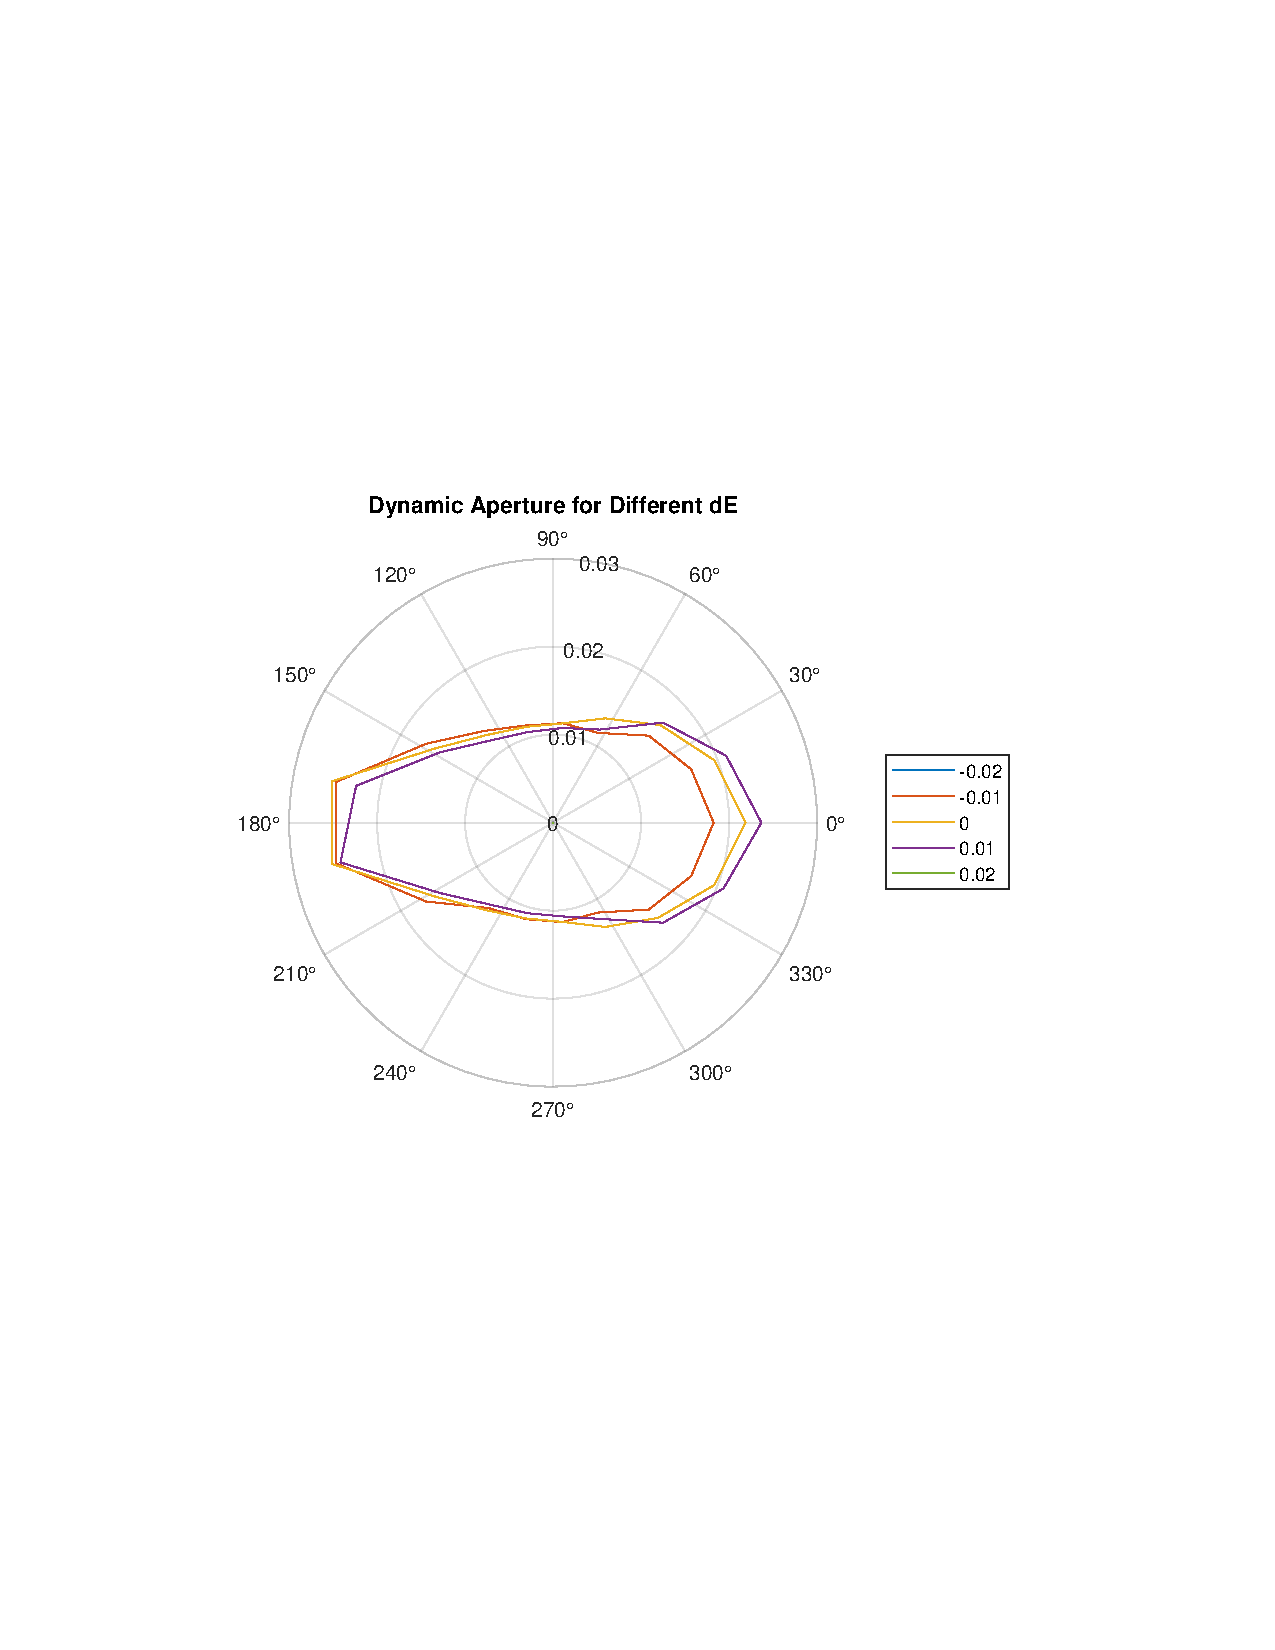
\includegraphics[width=1\linewidth]{da_sc_da_vs_de.pdf}
        \caption{Dynamic aperture for different energy deviations.}
    \end{figure}
\end{column}
\begin{column}{0.5\textwidth}
    \begin{itemize}
        \item Smaller aperture at higher deviations due to chromaticity effects.
        \item Symmetry observed around on-momentum (dE = 0).
    \end{itemize}
\end{column}
\end{columns}
\end{frame}

% Results - Angular Resolution Study
\begin{frame}{Results: Angular Resolution Study}
\begin{columns}
\begin{column}{0.5\textwidth}
    \begin{figure}
        \centering
        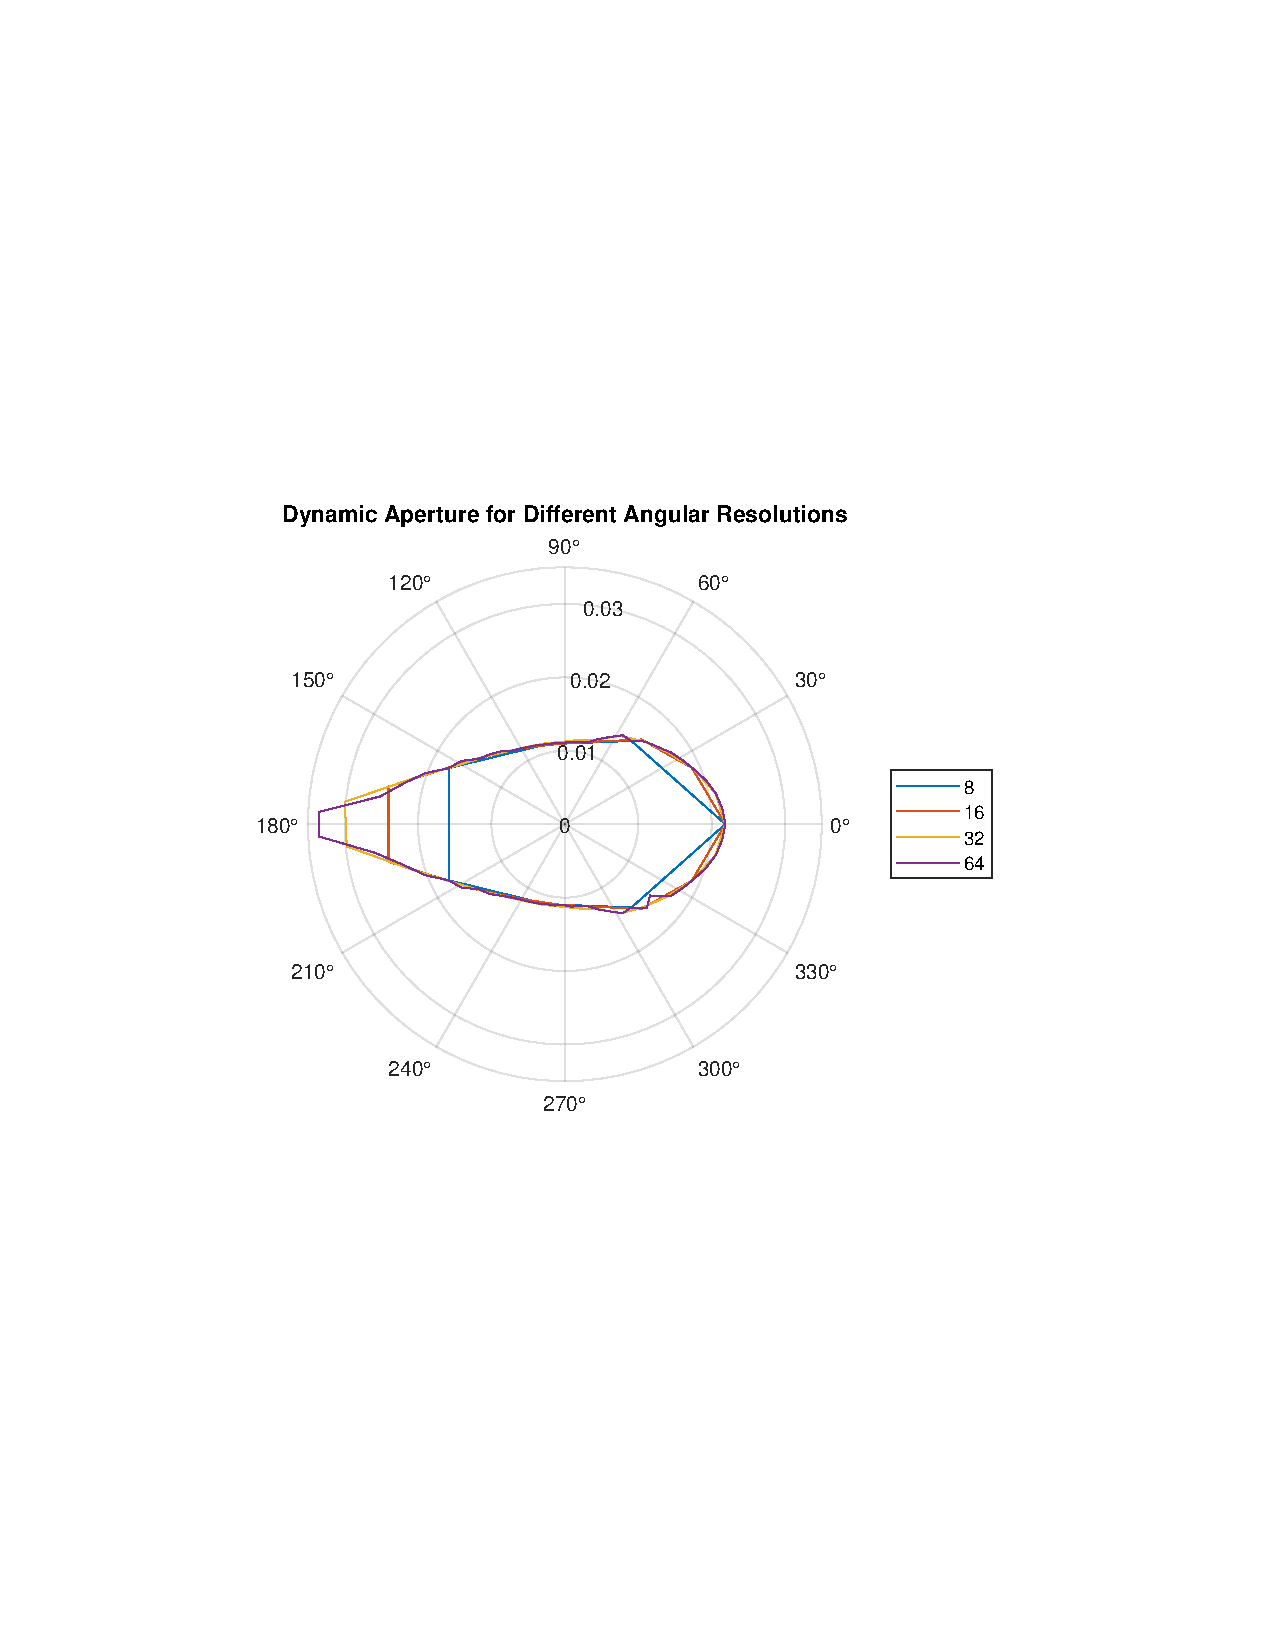
\includegraphics[width=1\linewidth]{sc_da_vs_cntangle.pdf}
        \caption{Aperture shapes with varying angular resolutions.}
    \end{figure}
\end{column}
\begin{column}{0.5\textwidth}
    \begin{itemize}
        \item Higher resolution shows detailed shape.
        \item Computational cost increases with resolution.
    \end{itemize}
\end{column}
\end{columns}
\end{frame}

% Results - Lattice Element Impact
%\begin{frame}{Results: Lattice Element Impact}
%    \begin{figure}
%        \centering
%        \includegraphics[width=0.7\linewidth]{figures/quadrupole_strength.png}
%        \caption{Effect of quadrupole strength variation on dynamic aperture.}
%    \end{figure}
%    \begin{itemize}
%        \item Dynamic aperture sensitive to quadrupole settings.
%        \item Potential for optimizing stability by fine-tuning.
%    \end{itemize}
%\end{frame}

\begin{frame}{Results: Long-Term Stability Checks}
\begin{columns}
\begin{column}{0.5\textwidth}
 \begin{figure}
    \centering
    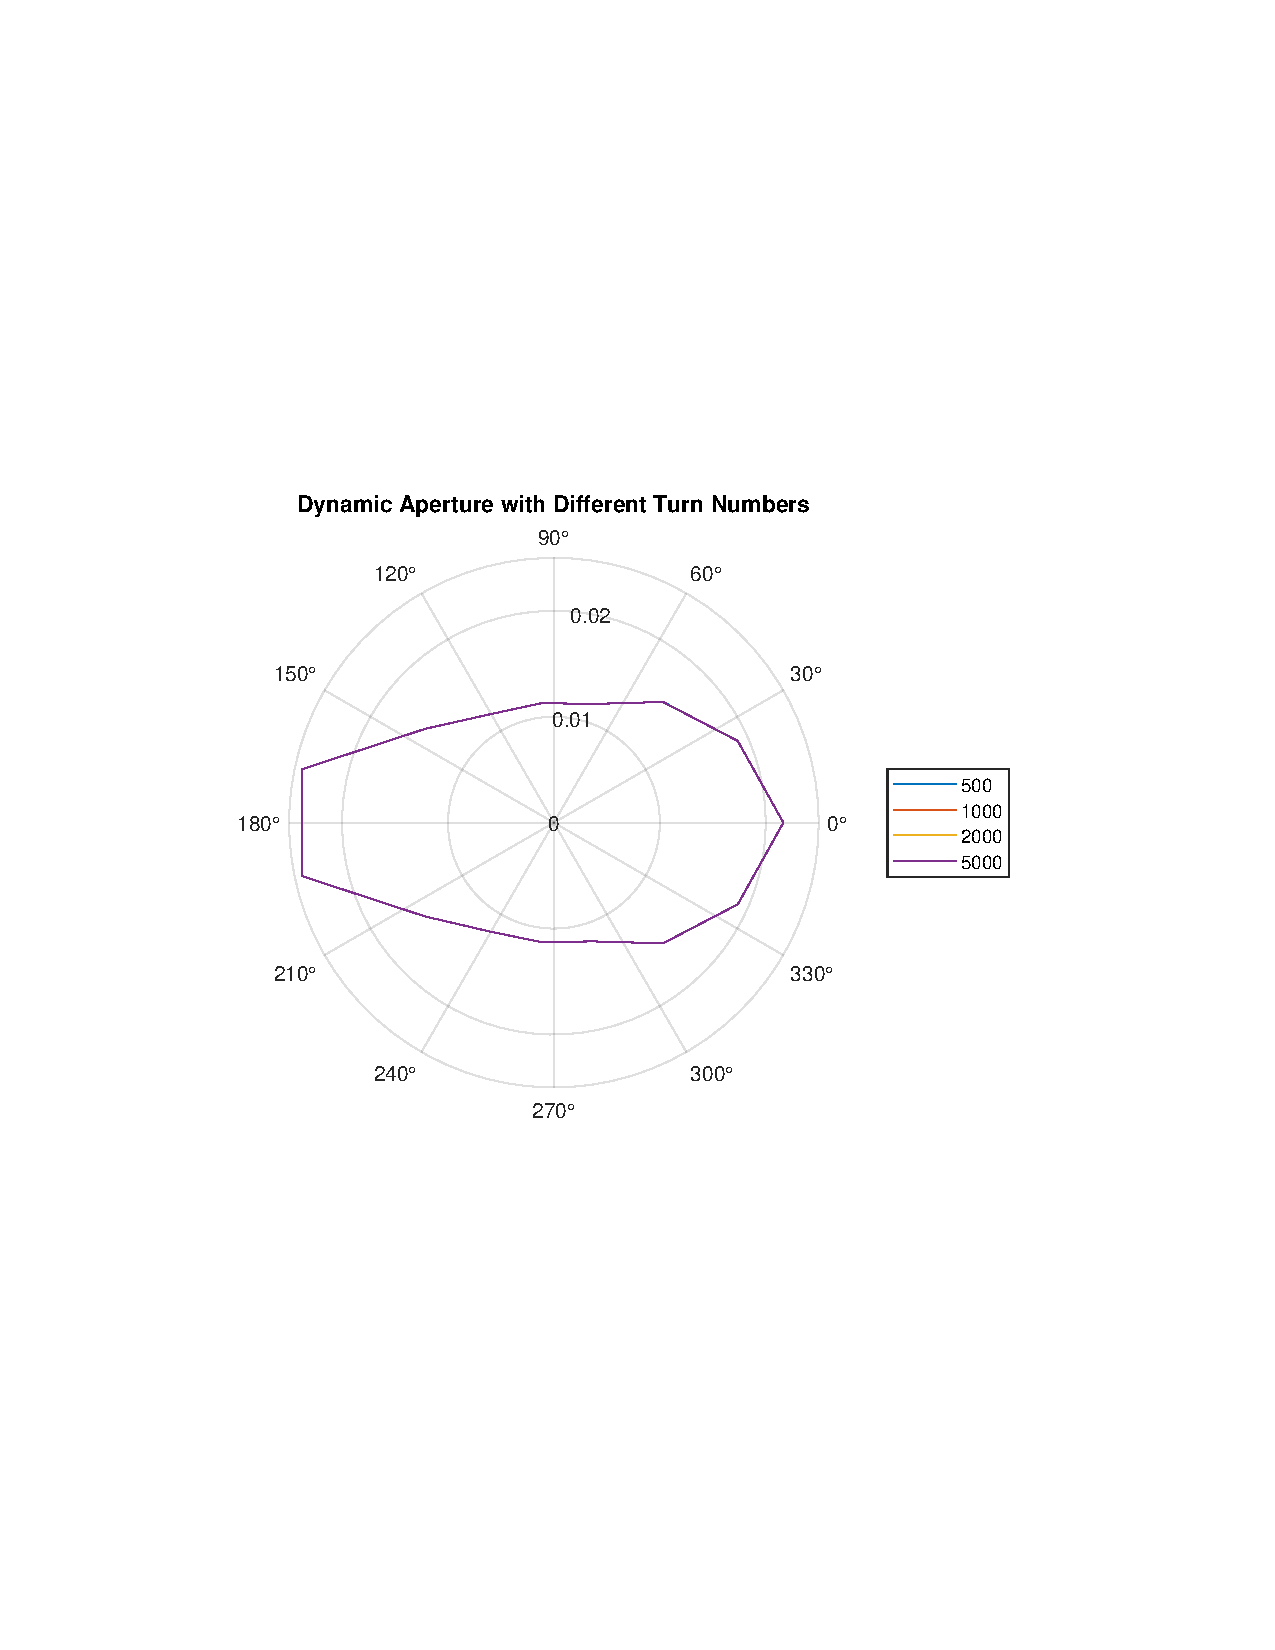
\includegraphics[width=1\linewidth]{sc_da_vs_nturn.pdf}
    \caption{Investigate long-term stability by varying the number of turns }
 \end{figure}
\end{column}
\begin{column}{0.5\textwidth}


\end{column}
\end{columns}
\end{frame}

% Discussion
\begin{frame}{Discussion}
    \begin{itemize}
        \item Off-momentum particles affect the aperture asymmetrically.
        \item Angular resolution impacts the accuracy of the shape.
        \item Quadrupole strengths significantly influence stability.
    \end{itemize}
\end{frame}

% Conclusion
\begin{frame}{Conclusion and Future Work}
    \begin{itemize}
        \item Dynamic aperture provides insights into particle stability.
        \item Nonlinearities and lattice imperfections influence results.
        \item Future work:
        \begin{itemize}
            \item Investigate nonlinear elements (sextupoles, octupoles).
            \item Compare with experimental measurements.
            \item Optimize using advanced algorithms.
        \end{itemize}
    \end{itemize}
\end{frame}

% References
\begin{frame}{References}
    \begin{thebibliography}{10}
        \beamertemplatetextbibitems
        \bibitem{bib:SCdynAperture}
        T. Hellert et al., \textit{Lattice correction and commissioning simulation of the Advanced Light Source upgrade storage ring}, Phys. Rev. Accel. Beams 25/110701, 2022.
    \end{thebibliography}
\end{frame}

\end{document}

